% !TeX spellcheck = pl_PL
\documentclass[a4paper,twoside]{article}
\usepackage{polski}
\usepackage[utf8]{inputenc}
\usepackage{graphicx}
\usepackage{amsmath}

\usepackage[unicode, bookmarks=true]{hyperref} %do zakładek
\usepackage{tabto} % do tabulacji
\NumTabs{6} % globalne ustawienie wielkosci tabulacji
\usepackage{array}
\usepackage{multirow}
\usepackage{array}
\usepackage{dcolumn}
\usepackage{bigstrut}
\usepackage{color}
\usepackage[usenames,dvipsnames]{xcolor}
\usepackage{svg}
\usepackage{xfrac}
\usepackage{floatrow}

\usepackage{multirow,tabularx}
\newcolumntype{Y}{>{\centering\arraybackslash}X}
\renewcommand{\arraystretch}{2}

% === Reset inkrementacji sekcji przy nowym parcie === %
\usepackage{titlesec}

\makeatletter
\@addtoreset{section}{part}
\makeatother
\titleformat{\part}[display]
{\normalfont\LARGE\bfseries\centering}{}{-60pt}{}

% === Dodanie krpki do sekcji
\titlelabel{\thetitle.\quad}


\setlength{\textheight}{24cm}
\setlength{\textwidth}{15.92cm}
\setlength{\footskip}{10mm}
\setlength{\oddsidemargin}{0mm}
\setlength{\evensidemargin}{0mm}
\setlength{\topmargin}{0mm}
\setlength{\headsep}{5mm}

\setlength{\textfloatsep}{10pt plus 1.0pt minus 2.0pt}


\begin{document}
\bibliographystyle{plain}

% ************************************************************
% --- Strona tytułowa
% ************************************************************
\begin{titlepage}
	\begin{table}[htbp]
		\centering
		\begin{tabular}{|c|c|c|c|c|c|c|}
			\hline
			\multicolumn{7}{|c|}{\textbf{{\LARGE Projekt programistyczny}}} \bigstrut\\[4pt]
			\hline
			Rok akademicki & Termin & Rodzaj studiów & Kierunek & Prowadzący & Grupa & Sekcja \bigstrut\\
			\hline
			\multicolumn{1}{|c|}{\multirow{2}[4]{*}{{\large 2014/2015}}} & \multicolumn{1}{c|}{{\large Wtorek}} & \multicolumn{1}{c|}{\multirow{2}[4]{*}{{\large SSI}}} & \multicolumn{1}{c|}{\multirow{2}[4]{*}{{\large INF}}} & \multicolumn{1}{c|}{\multirow{2}[4]{*}{\begin{tabular}{@{}c@{}}{\large dr inż.} \\[-9pt] {\large Arkadiusz}\\[-9pt] {\large Biernacki}\end{tabular}}} & \multicolumn{1}{c|}{\multirow{2}[4]{*}{{\large GKiO3}}} & \multicolumn{1}{c|}{\multirow{2}[4]{*}{{\large 1}}} \bigstrut\\
			\cline{2-2}    \multicolumn{1}{|c|}{} & \multicolumn{1}{c|}{{\large 12:45 - 15:00}} & \multicolumn{1}{c|}{} & \multicolumn{1}{c|}{} & \multicolumn{1}{c|}{} & \multicolumn{1}{c|}{} & \multicolumn{1}{c|}{} \bigstrut\\
			\hline
		\end{tabular}%
	\end{table}%
	
	\centering
	
\includegraphics[width=0.6\textwidth]{./images/logo.png}
	\\\vspace{10mm}
	\textbf{{\huge Karta projektu}}\\\vspace{5mm}
	\textbf{{\Huge Danmaku Shooter}}
	\\
	\vfill
	\begin{flushright}
			{\Large \textbf{Skład sekcji}:}\\
		\begin{tabular}{rr}
			{\Large Buchała} & {\Large Bartłomiej}\\[-3pt]
			{\Large Forczmański} & {\Large Mateusz}\\[-3pt]
			{\Large Motyka} & {\Large Marek}\\[-3pt]
			{\Large Wudecki} & {\Large Wojciech}
		\end{tabular}
	\end{flushright}
	
\end{titlepage}



% ************************************************************
% --- Strona z założeniami
% ************************************************************
\part{\huge \textbf{Krótki opis aplikacji}}
\textit{Shoot' em up} (w skrócie zwany shmup) jest gatunkiem gier akcji wywodzącym się w prostej linii od gier typu \textit{Space Invaders} lub \textit{River Raid}. Kontrolowana przez gracza postać (np. statek) w pojedynkę stawia czoło przeciwnikom, niszcząc ich za pomocą wystrzeliwanych pocisków, jednocześnie unikając ich ataków. Podgatunek shmupów, zwany \textit{danmaku} (z jap. \textit{ściana pocisków} lub \textit{piekło pocisków}) kładzie większy nacisk na omijanie wrogich ataków, niż na ofensywie. Przykładowymi danmaku są np. \textit{Ikaruga} czy większość gier z uniwersum \textit{Touhou Project}. \\

Gra powstawać będzie jako projekt łączony z przedmiotów Projekt Programistyczny i Grafika Komputerowa.

% TO DO: Insert 9000 godzin w Paincie. % 

\begin{center}
	\fbox{%
		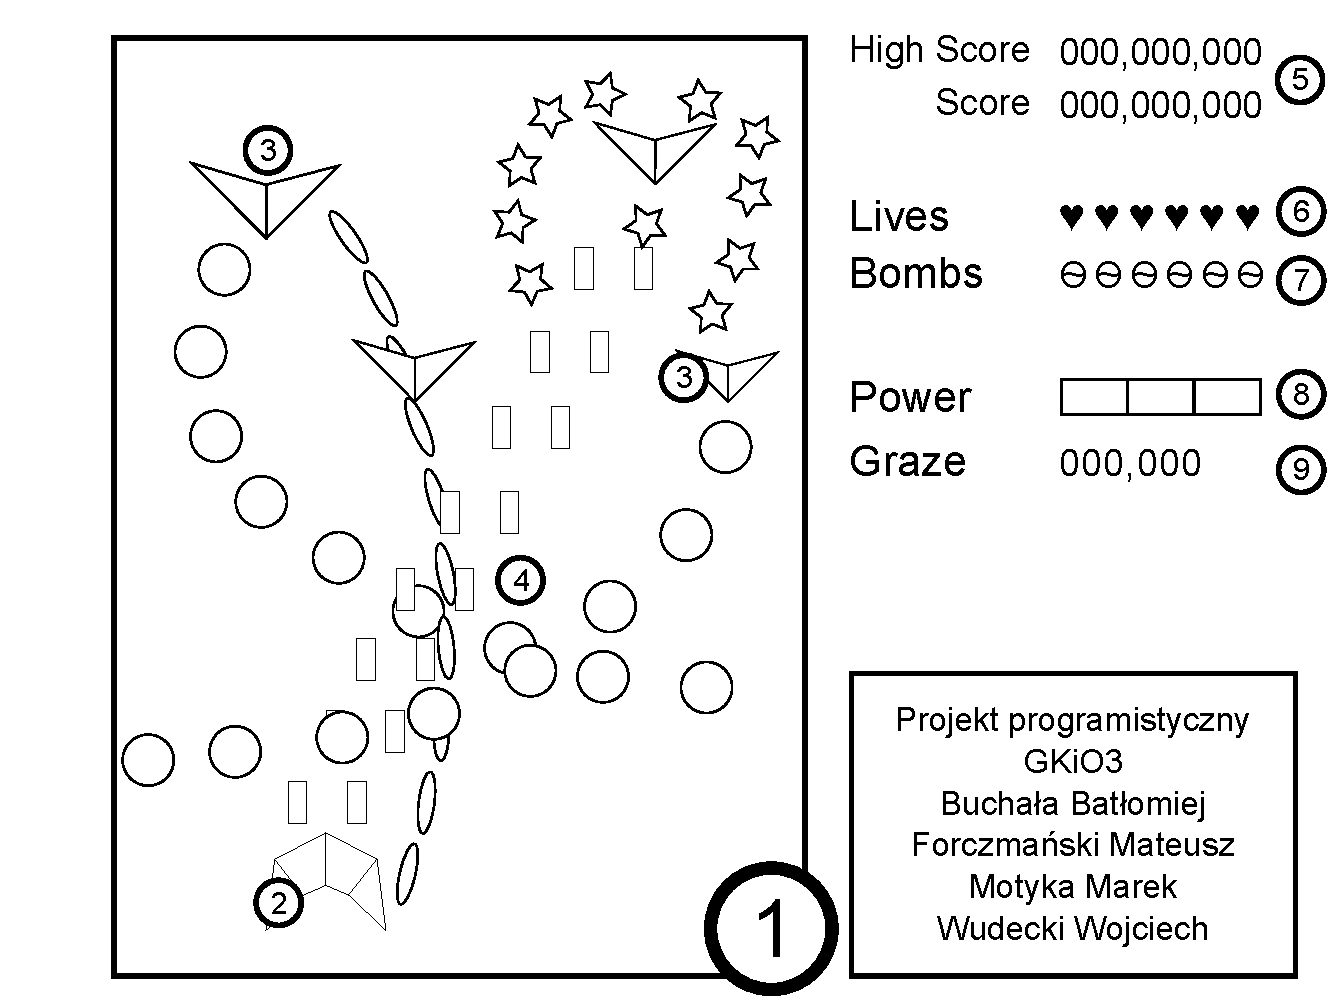
\includegraphics[width=0.8\textwidth]{./images/screen01}%
	}
	\vspace{5pt}
\end{center}
\begin{enumerate}
	\item Ekran gry właściwej. W jej obrębie znajduje się gracz, pociski oraz wszyscy wrogowie. 
	\item Grywalna postać, porusza się po ekranie gry, unikając pocisków oraz strzelając do wrogów.
	\item Wrogowie, których należy pokonać.
	\item Chmara pocisków. Jak widać na rysunku, nie wchodzą ze sobą w żadną interakcję, każdy leci swoim wyznaczonym torem. Sprajty wrogów są niewrażliwe na swoje pociski, nie występuje \textit{friendly fire}.
	\item Liczba zdobytych punktów oraz porównywanie ich z największym wynikiem.
	\item Liczba pozostałych żyć. W trakcie gry można zdobywać kolejne. Utrata wszystkich kończy grę.
	\item Liczba pozostałych bomb. Każda wykorzystana bomba zapewnia kilkusekundową odporność na wrogie pociski oraz umożliwia pojedynczy silniejszy atak. Można je zdobyć w trakcie gry.
	\item Pasek mocy, napełnia się w trakcie gry wraz ze zdobytymi punktami. Utrata życia skutkuje zmniejszeniem paska o 1 segment.
	\item Liczba "otarć", czyli uniknięć bardzo blisko pocisku. Aby umożliwić większe wyzwanie, ostateczny wynik pomnożony jest przez licznik Graze.
\end{enumerate}


% Piekło pocisków brzmi jak Mikołów. Jesteś sobie taki biedny ty, a obok Ciebie Raku i Korda i Ci co chwilę pociskają ;_; %

% Zostawiam póki co takie wykastrowane, dopóki nie ustalimy więcej szczegółów. W ostateczności można tak zostawić, bo to ma być króciutki zarys. %

\newpage

\part{\huge \textbf{Założenia projektowe}}

\section{Narzędzie do modelowania UML}

{\Large Enterprise Architect} \\\\
Jest to narzędzie, który poznaliśmy semestr wcześniej na projekcie z przedmiotu Inżynieria Oprogramowania. Ponieważ ww. przedmiot kładł bardzo duży nacisk na modelowanie diagramów, większość z nas jest z nim dobrze zaznajomiona. Przejrzystość tego programu może być niezwykle przydatna podczas tworzenia np. diagramu przypadków użycia. Równolegle wykorzystujemy EA do stworzenia diagramów UML dla projektu z przedmiotu Bazy Danych II.

\section{System kontroli wersji}

{\Large GitHub} \\\\
Jest to bardzo powszechnie stosowane narzędzie wśród deweloperów pracujących w grupach. Jego zaletami jest m.in. klient aplikacji na system operacyjny Windows, łatwy do przyswojenia i intuicyjny interfejs i łatwość w zarządzaniu starszymi wersjami. Podobnie jak w przypadku Enterprise Architecta, większość z nas miała już wcześniej styczność z GitHubem i korzysta z niego od pewnego czasu.

\section{Narzędzia pracy grupowej}

{\Large Facebook/Skype/Gmail} \\\\
W celu ułatwienia komunikacji wykorzystane zostaną popularne sieci społecznościowe oraz komunikatory. Ułatwi nam to wspólną współpracę jak i dzielenie się pomysłami oraz dokonanymi zmianami.
% Takie cuś jest na platformie do opisania. Chyba chodzi o komunikatory. GG, Facebook, Skype? Wuda jako środek transportu do kumpla się liczy? :P %
%  "Samochód jako miejce dyskusji i źródło inspiracji" %
\section{Środowisko programistyczne}

{\Large Microsoft Visual Studio 2012} \\\\
Wybraliśmy to środowisko ze względu na przyjazny interfejs, który nawet w najtrudniejszych sytuacjach potrafi okazać się bardzo pomocny. Pracujemy na nim od dłuższego czasu co ułatwi nam szybki dostęp do potrzebnych narzędzi. Etap debugowania posiada wiele możliwości kontroli naszego programu, co na pewno pozwoli uniknąć kilku czasochłonnych błędów. Ponieważ czasami pojawiają się problemy w kompilacji związane z różnymi wersjami VS, wspólnie wybraliśmy jedną wersję środowiska w celu usunięcia tych przeszkód.

\section{Język programowania}

{\Large C++ / C\#} \\\\
Głównym kryterium wyboru tych języków był wysoki poziom integracji z platformą programistyczną .NET oraz środowiskiem programistycznym Microsoft Visual Studio. Dzięki temu możemy uniknąć problemów podczas łączenia poszczególnych komponentów naszego projektu. Dodatkowo, język C++ poznaliśmy wcześniej na przedmiocie Programowanie Komputerów, a także używaliśmy go na innych laboratoriach - posiadamy pewne doświadczenie w tworzeniu aplikacji z jego użyciem. Język C\# jest nieco bardziej zaawansowane i na jego użycie zdecydujemy się wtedy, gdy opanujemy go na odpowiednim poziomie.

\section{Biblioteka graficzna}
{\Large DirectX} \\\\
Nasze doświadczenie z zaawansowanymi bibliotekami nie jest duże, w trakcie zajęć z programowania korzystaliśmy z takich rozwiązań jak SFML 2.0 lub Allegro, jednak w ramach tego projektu zdecydowaliśmy się na coś większego. Wybór padł na DirectX, który jest nastawiony na programowanie zorientowane obiektowo oraz jest wspierane przez Visual Studio w postaci szablonów i dodatków.

\section{Platforma programistyczna}
{\Large .NET Framework} \\\\
W typ przypadku ponownie zadecydowała integracja z innymi produktami od Microsoftu (VS, język C\#) oraz fakt, że firma parę miesięcy temu udostępniła platformę na zasadach Open Source.


\end{document}